\section{Trasformata di Burrows-Wheeler}
\label{secbwt}
Introdotta nel 1994 da Burrows e Wheeler con lo scopo di comprimere testi, la
\textbf{Burrows-Wheeler Transform} ($\BWT$) \cite{bwt} è divenuta ormai uno
standard nel 
campo dell'algoritmica su stringhe e della bioinformatica,
grazie ai suoi molteplici vantaggi sia dal punto di vista della complessità
temporale che da quello dell'efficienza in memoria.\\
Nel dettaglio la $\BWT$ è una trasformata reversibile che
permette una compressione lossless, quindi senza perdita
d'informazione. Tale trasformazione viene costruita a partire dal riordinamento
dei caratteri del testo in input, riordinando lessicograficamente le cosiddette
\textit{rotazioni} del testo. Interessante è la proprietà per cui caratteri
uguali tendono ad essere posti consecutivamente all'interno della stringa
prodotta dalla trasformata. Questa proprietà è causata dalle ripetizioni di
sottostringhe all'interno del testo stesso.
\begin{definizione}
  Dato un testo $T$ \$-terminato, tale che $|T|=n$, si definisce la
  Burrows--Wheeler Transform di $T$, denotata con
  $\BWT_T$, come un array di caratteri lungo $n$ dove l'elemento $i$-esimo è il
  carattere che precede l'$i$-esimo suffisso $T$ nel riordinamento
  lessicografico. Più formalmente si ha che:
  \begin{equation}
    \label{eq:bwt1}
    \BWT_T[i]=
    \begin{cases}
      T[\SA_T[i]-1]&\mbox{ se } \SA_T[i]\neq 1\\
      \$&\mbox{ altrimenti}
    \end{cases},\,\, \forall\, i\in\{0,n-1\}
  \end{equation}
\end{definizione}
In termini operativi, la $\BWT$ di un testo è calcolabile riordinando
lessicograficamente tutte le possibili rotazioni del testo $T$.
\begin{definizione}
  Si definisce rotazione $i$-esima di
  un testo $T$ lungo $n$, denotata con $\ROT_T(i)$, come la stringa ottenuta
  dalla concatenazione 
  del suffisso $i$-esimo con la restante porzione del testo. Più formalmente si
  ha che, denotando con $X\cdot Y$ la concatenazione tra
  la stringa $X$ e la stringa $Y$:
  \begin{equation}
    \label{eq:bwt2}
    \ROT_T(i)=T[i,n-1]\cdot T[0,i-1],\,\,\forall\, i\in\{0,n-1\}
  \end{equation}
\end{definizione}
Data questa definizione, quindi, la $\BWT$ del testo $T$ risulta essere
l'ultima colonna della matrice, detta \textbf{Burrows--Wheeler Matrix} ($\BWM$),
che si ottiene riordinando tutte le  
rotazioni di $T$, che altro non sono che i suffissi già riordinati per
il calcolo di $\SA_T$ a cui viene concatenata la parte restante del
testo.\\
Un altro array spesso utilizzato insieme alla $\BWT$ è il cosiddetto
array $\F$, lungo $|T|$, che è l'array formato
dalla prima colonna della $\BWM$. In pratica l'array $\F_T$ è,
banalmente, l'array formato dal riordinamento 
lessicografico dei caratteri del testo $T$.
\begin{esempio}
  Si prenda la stringa:
  \[s=\mbox{mississippi\$},\,\,|s|=12\]
  Si produce la $\BWM_T$, da cui si estraggono $\F_T$ e $\BWT_T$:
  \begin{table}[H]
    \centering
    \footnotesize
    \begin{tabular}{c|c|c|c|c} 
      \textbf{Indice} & $\SA_T$ & $\F_T$ & $\BWM_T$
      & $\BWT_T$\\ 
      \hline
      0 & 11 & \$ & \$mississippi & i\\
      1 & 10 & i & i\$mississipp & p\\
      2 & 7 & i & ippi\$mississ & s\\
      3 & 4 & i & issippi\$miss & s\\
      4 & 1 & i & ississippi\$m & m\\
      5 & 0 & m & mississippi\$ & \$\\
      6 & 9 & p & pi\$mississip & p\\
      7 & 8 & p & ppi\$mississi & i\\
      8 & 6 & s & sippi\$missis & s\\
      9 & 3 & s & sissippi\$mis & s\\
      10 & 5 & s & ssippi\$missi & i\\
      11 & 2 & s & ssissippi\$mi & i\\
    \end{tabular}
  \end{table}
\end{esempio}
L'importanza di questa trasformata è dovuta soprattutto al fatto che sia
reversibile, implicando quindi che, a partire da $\BWT_T$, sia possibile
ricostruire $T$. Questo è possibile grazie ad una proprietà intrinseca della
trasformata che viene riassunta nel concetto di \textbf{LF-mapping}.
\begin{definizione}
  Dato un testo $T$, tale che $|T|=n$, data la sua $\BWT_T$ e il suo array
  $\F_T$ 
  si definisce LF-mapping come la proprietà per la quale l'$i$-esima
  occorrenza di un carattere $\sigma$ in $\BWT_T$ corrisponde all'$i$-esima
  occorrenza dello stesso carattere in $\F_T$.
\end{definizione}
Grazie a questa definizione è possibile partire dall'ultimo carattere del testo,
ovvero $\sigma=\$$, e ricostruire l'intero testo a ritroso. Si vede quindi un
breve esempio. 
\begin{esempio}
  Si riprende l'esempio precedente, avendo:
  \[\BWT_T=\mbox{ipssm\$pissii}\mbox{ e }\F_T=\mbox{\$iiiimppssss}\]
  E avendo i seguenti caratteri associati dall'\textit{LF-mapping}:
  \begin{figure}[H]
    \centering
    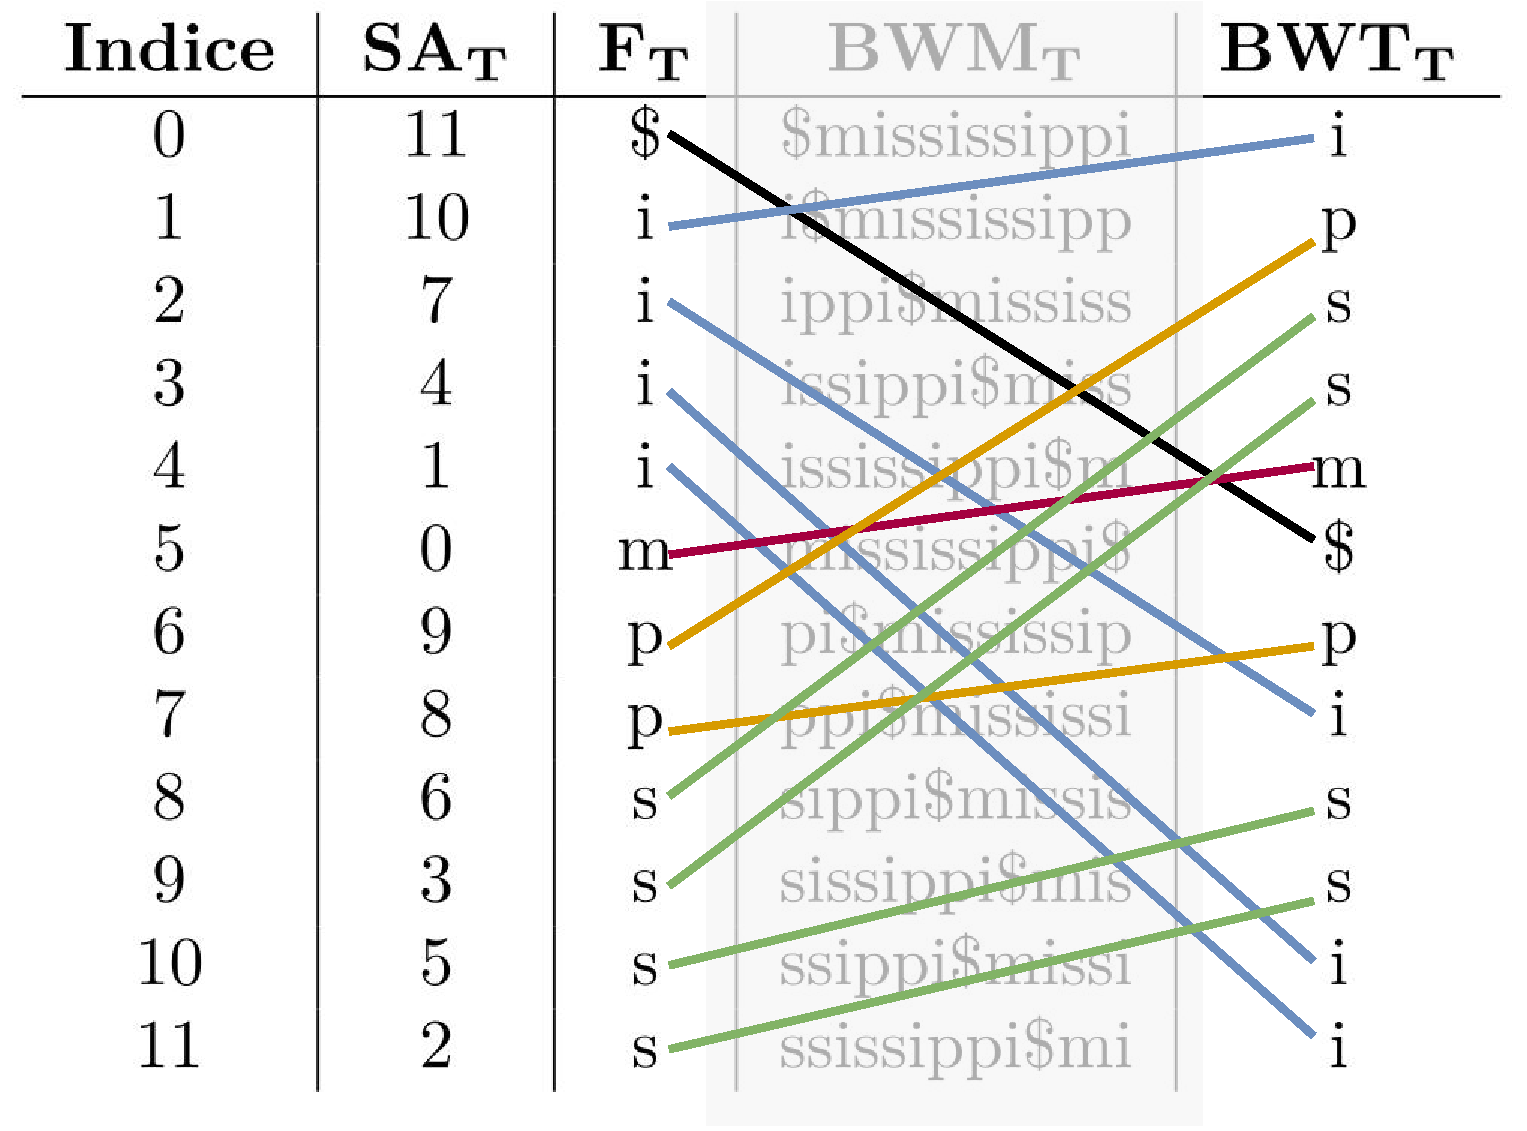
\includegraphics[scale = 0.33]{img/lf.pdf}
  \end{figure}
  Si comincia dal simbolo '\$' in $\BWT_T$, che è l'ultimo carattere di $T$. Si
  ha che esso corrisponde al primo e unico simbolo '\$' in $\F_T$, all'indice
  $0$. Tale simbolo, per l'ovvia proprietà delle rotazioni è preceduto dal
  simbolo $\BWT_T[0]=\mbox{'i'}$ in $T$. Quindi $\mbox{'i'}$ precederà '\$' in
  $T$:
  \[T=\ldots\mbox{i\$}\]
  Si sa inoltre che
  tale $\mbox{'i'}$ è il primo $\mbox{'i'}$ in $\BWT_T$. Si cerca quindi il
  primo simbolo $\mbox{'i'}$ anche in $\F_T$,
  sapendo che sono lo stesso simbolo nel testo. A questo punto il simbolo allo
  stesso indice di tale $\mbox{'i'}$ nella $\BWT_T$, ovvero il simbolo
  $\mbox{'p'}$, sarà il simbolo che precede $\mbox{'i'}$ nel testo:
  \[T=\ldots\mbox{pi\$}\]
  Proseguendo a ritroso si ricostruisce l'intero testo:
  \[T=\mbox{mississippi\$}\]
\end{esempio}
\dc{Questo esempio serve davvero?}
\subsubsection{FM-index}
Tramite l'uso dell'LF-mapping è possibile risolvere il problema di
ricerca di un pattern all'interno del testo, tramite l'algoritmo nominato
\textbf{backward search}. Questa tecnica consiste nell'iterare il pattern da
destra a sinistra e
salvare, di volta in volta, un intervallo sul suffix array. Nel
dettaglio, ipotizzando di essere in posizione $i$ del pattern, tale
intervallo è relativo a quei suffissi che hanno come prefisso il suffisso
$i$-esimo del pattern. Tale intervallo viene esteso usando il carattere
$P[i-1]$ selezionando il nuovo intervallo sul suffix array. Tale
aggiornamento è detto \textit{backward step} e consiste nell'aggiornare
l'intervallo sul suffix array a quei suffissi del testo che, estesi a sinistra
col carattere $(i-1)$-esimo del pattern, presentano un match con $P[i-1,
|P|-1]$.\\   
Usando la $\BWT$ è possibile usare due funzioni, dette $\C$ e $\Occ$, per
computare la backward search.
\begin{definizione}
  Dato un testo \$-terminato $T$, lungo $n$ e costruito su alfabeto $\Sigma$, si
  definisce la funzione $\C$, come una funzione:
  \begin{equation}
    \label{eq:bwt4}
    \C:\Sigma\cup \$\to \mathbb{N}
  \end{equation}
  Dato un carattere $\sigma\in\Sigma$, $\C(\sigma)$ restituisce il
  numero di 
  occorrenze dei caratteri lessicograficamente più piccoli di $\sigma$ in $T$.
\end{definizione}
\begin{definizione}
  Dato un testo \$-terminato $T$, lungo $n$ e costruito su alfabeto $\Sigma$, e
  la sua $BWT_T$, si definisce la funzione $\Occ$, come una funzione:
  \begin{equation}
    \label{eq:bwt5}
    \Occ:\Sigma\cup \$\times \{0,n\}\to \mathbb{N}
  \end{equation}
  Dato un carattere $\sigma\in\Sigma$ e una posizione $i$ della
  $BWT_T$, $\Occ(\sigma,i)$ restituisce il numero di occorrenze del carattere
  $\sigma$ nei primi $i$ elementi di $\BWT_T$.
\end{definizione}
Questa coppia di funzioni prende il nome di \textbf{FM-index} \cite{fm}, il
quale è definito essere un self index in quanto è possibile tenere in
memoria solo tale indice per ottenere i risultati medesimi della $\BWT_T$,
ricordando anche che da essa si può ricostruire il testo $T$.
\begin{esempio}
  Si prenda la stringa:
  \[T=\mbox{mississippi\$},\,\,|s|=12\]
  Che produce:
  \[\BWT_T=\mbox{ipssm\$pissii}\]
  Si ha, per $\C(\sigma)$:
  \begin{table}[H]
    \centering
    \begin{tabular}{c||c}
      $\sigma$ & $\C(\sigma)$\\
      \hline
      \hline
      \$ & 0\\
      i & 1 \\
      m & 5\\
      p & 6\\
      s & 8\\
    \end{tabular}
  \end{table}
  Per $\Occ(\sigma, i)$, si ha:
  \begin{table}[H]
    \centering
    \begin{tabular}{c||c|c|c|c|c}
      0 & 0 & 0 & 0 & 0 & 0 \\
      1 & 0 & 1 & 0 & 0 & 0 \\
      2 & 0 & 1 & 0 & 1 & 0 \\
      3 & 0 & 1 & 0 & 1 & 1 \\
      4 & 0 & 1 & 0 & 1 & 2 \\
      5 & 0 & 1 & 1 & 1 & 2 \\
      6 & 1 & 1 & 1 & 1 & 2 \\
      7 & 1 & 1 & 1 & 2 & 2 \\
      8 & 1 & 2 & 1 & 2 & 2 \\
      9 & 1 & 2 & 1 & 2 & 3 \\
      10 & 1 & 2 & 1 & 2 & 4 \\
      11 & 1 & 3 & 1 & 2 & 4 \\
      12 & 1 & 4 & 1 & 2 & 4 \\
      \hline
      \hline
      i/$\sigma$ & \$ & i & m & p & s
    \end{tabular}
  \end{table}
\end{esempio}
Dato un simbolo $\sigma$ del pattern e il precedente intervallo $[f,g)$ su
$\SA_T$, si esegue il backward step, tramite l'FM-index,
aggiornando $f$ e $g$ nel seguente modo: 
\begin{equation}
  \label{eq:bwt6}
  f'=\C(\sigma)+\Occ(\sigma, f),\quad g'=\C(\sigma)+\Occ(\sigma, g)
\end{equation}
Ritornando il nuovo intervallo $[f, g)\gets [f', g')$ sse $f'< g'$.
Si segnala che tali variabili sono inizializzate con $f=0$ e $g=n$.\\
Tale calcolo altro non è che l'LF-mapping. Infatti, partendo da un
intervallo su $\SA_T$ (che è anche un intervallo su $\BWT_T$), si identificano
quali suffissi sono preceduti dal simbolo del pattern voluto. Tale simbolo, se
il 
pattern ha un'occorrenza fino al carattere in analisi, sarà presente in
sottointervallo di $[f,g)$ sulla $\BWT_T$. Una volta identificati tali caratteri
su $\BWT_T$ si usano $\C(\sigma)$ e $\Occ(\sigma, i)$, per trovare tali
caratteri su $\F_T$, calcolando il nuovo intervallo $[f,g)$.
\dc{capire se dire meglio}
\begin{esempio}
  Si assuma il pattern $P=\mbox{iss}$ da voler ricercare nel testo
  $T=\mbox{mississippi\$}$. 
  Si ha, in termini di inizializzazione che $f=0$, $g=12$,
  $\sigma=P[|P|-1]=P[2]=s$. Si calcolano i nuovi $f'$ e $g'$:
  \[f'=\C(s)+\Occ(s, 0)=8+0=8\]
  \[g'=\C(s)+\Occ(s, 12)=8+4=12\]
  Ottenendo l'intervallo $[8,12)$ sul suffix array.\\
  Si prosegue leggendo il carattere $\sigma=P[1]=s$:
  \[f'=\C(s)+\Occ(s, 8)=8+2=10\]
  \[g'=\C(s)+\Occ(s, 12)=8+4=12\]
  Limitando quindi l'intervallo a $[10,12)$. Si noti che tale intervallo
  corrisponde ai due simboli ``s'' presenti in $\BWT_T[8,11]$, che sono
  esattamente i simboli in $\F_T[10,11]$.
  Un ulteriore aggiornamento, col carattere $\sigma=P[0]=i$, comporta:
  \[f'=\C(i)+\Occ(i, 10)=1+2=3\]
  \[g'=\C(i)+\Occ(i, 12)=1+4=5\]
  Avendo l'intervallo finale su $\SA_T$ del match, ovvero: $[3,5)$.
  Seguendo l'intero ragionamento sul \textit{suffix array} si avrebbe:
  \begin{table}[H]
    \centering
    \scriptsize
    \begin{tabular}{c|c|c|c|c} 
      \textbf{Indice} & $\SA_T$ & $\F_T$ & $\BWM_T$
      & $\BWT_T$\\ 
      \hline
      {\color{nordred}{0}} & 11 & \$ & {\color{nordred}{\$}}mississippi & i\\
      {\color{nordred}{1}} & 10 & i & {\color{nordred}{i}}\$mississipp & p\\
      {\color{nordred}{2}} & 7 & i & {\color{nordred}{i}}ppi\$mississ
      & {\color{nordgreen}{s}}\\
      {\color{nordred}{3}} & 4 & i & {\color{nordred}{i}}ssippi\$miss
      & {\color{nordgreen}{s}}\\
      {\color{nordred}{4}} & 1 & i & {\color{nordred}{i}}ssissippi\$m & m\\
      {\color{nordred}{5}} & 0 & m & {\color{nordred}{m}}ississippi\$ & \$\\
      {\color{nordred}{6}} & 9 & p & {\color{nordred}{p}}i\$mississip & p\\
      {\color{nordred}{7}} & 8 & p & {\color{nordred}{p}}pi\$mississi & i\\
      {\color{nordred}{8}} & 6 & s & {\color{nordred}{s}}ippi\$missis
      & {\color{nordgreen}{s}}\\
      {\color{nordred}{9}} & 3 & s & {\color{nordred}{s}}issippi\$mis
      & {\color{nordgreen}{s}}\\
      {\color{nordred}{10}} & 5 & s & {\color{nordred}{s}}sippi\$missi & i\\
      {\color{nordred}{11}} & 2 & s & {\color{nordred}{s}}sissippi\$mi & i\\
    \end{tabular}
    $\implies$
    \begin{tabular}{c|c|c|c|c} 
      \textbf{Indice} & $\SA_T$ & $\F_T$ & $\BWM_T$
      & $\BWT_T$\\  
      \hline
      0 & 11 & \$ & \$mississippi & i\\
      1 & 10 & i & i\$mississipp & p\\
      2 & 7 & i & ippi\$mississ & s\\
      3 & 4 & i & issippi\$miss & s\\
      4 & 1 & i & ississippi\$m & m\\
      5 & 0 & m & mississippi\$ & \$\\
      6 & 9 & p & pi\$mississip & p\\
      7 & 8 & p & ppi\$mississi & i\\
      {\color{nordred}{8}} & 6 & s & {\color{nordred}{s}}ippi\$missis
      & {\color{nordgreen}{s}}\\
      {\color{nordred}{9}} & 3 & s & {\color{nordred}{s}}issippi\$mis
      & {\color{nordgreen}{s}}\\
      {\color{nordred}{10}} & 5 & s & {\color{nordred}{s}}sippi\$missi & i\\
      {\color{nordred}{11}} & 2 & s & {\color{nordred}{s}}sissippi\$mi & i\\
    \end{tabular}
  \end{table}
  \[\Downarrow\]
  \begin{table}[H]
    \centering
    \scriptsize
    \begin{tabular}{c|c|c|c|c} 
    \textbf{Indice} & $\SA_T$ & $\F_T$ & $\BWM_T$
      & $\BWT_T$\\ 
      \hline
      0 & 11 & \$ & \$mississippi & i\\
      1 & 10 & i & i\$mississipp & p\\
      2 & 7 & i & ippi\$mississ & s\\
      3 & 4 & i & issippi\$miss & s\\
      4 & 1 & i & ississippi\$m & m\\
      5 & 0 & m & mississippi\$ & \$\\
      6 & 9 & p & pi\$mississip & p\\
      7 & 8 & p & ppi\$mississi & i\\
      8 & 6 & s & sippi\$missis & s\\
      9 & 3 & s & sissippi\$mis & s\\
      {\color{nordred}{10}} & 5 & s & {\color{nordred}{ss}}ippi\$missi
      & {\color{nordgreen}{i}}\\
      {\color{nordred}{11}} & 2 & s & {\color{nordred}{ss}}issippi\$mi
      & {\color{nordgreen}{i}}\\
    \end{tabular}
    $\implies$
    \begin{tabular}{c|c|c|c|c} 
      \textbf{Indice} & $\SA_T$ & $\F_T$ & $\BWM_T$
      & $\BWT_T$\\ 
      \hline
      0 & 11 & \$ & \$mississippi & i\\
      1 & 10 & i & i\$mississipp & p\\
      2 & 7 & i & ippi\$mississ & s\\
      {\color{nordred}{3}} & {\color{nordgreen}{\underline{4}}} & i
                                        & {\color{nordred}{iss}}ippi\$miss & s\\
      {\color{nordred}{4}} & {\color{nordgreen}{\underline{1}}} & i
                                        & {\color{nordred}{iss}}issippi\$m & m\\
      5 & 0 & m & mississippi\$ & \$\\
      6 & 9 & p & pi\$mississip & p\\
      7 & 8 & p & ppi\$mississi & i\\
      8 & 6 & s & sippi\$missis & s\\
      9 & 3 & s & sissippi\$mis & s\\
      10 & 5 & s & ssippi\$missi & i\\
      11 & 2 & s & ssissippi\$mi & i\\
    \end{tabular}
  \end{table}
  Avendo quindi che le occorrenze del pattern $P=\mbox{iss}$ iniziano alle
  posizioni $\SA_T[3]=4$ e $\SA_T[4]=1$ del testo.
\end{esempio}
\section{Trasformata di Burrows--Wheeler run-length encoded}
Come già introdotto, la $\BWT$ tende ad avere caratteri uguali in
posizioni consecutive all'interno della sua sequenza. Si è quindi 
pensato, fin da subito, ad un modo efficiente per memorizzare in modo compresso
testi mediante l'uso del run-length encoding. Tale tecnica consiste nel
memorizzare le cosiddette run, ovvero sequenze massimali di caratteri
uguali, mediante coppie: 
\[(\mbox{carattere}, \mbox{lunghezza della run})\]
\begin{esempio}
  Vediamo un breve esempio.\\
  Si ipotizzi di avere la seguente stringa:
  \[s=\mbox{aaaacctgggggg}\]
  Una sua memorizzazione run-length sarebbe del tipo:
  \[\{(a,4),(c,2),(t,1),(g,6)\}\]
\end{esempio}
\subsection{RLBWT e r-index}
In questa direzione, nel 2005, M\"{a}niken e Navarro proposero la
\textbf{Run-Length encoded Burrows-–Wheeler Transform} ($\RLBWT$)
\cite{rlbwt}.
\begin{definizione}
  Dato un testo $T$ si definisce la \RLBWT di $T$
  come la rappresentazione run-length encoded della $\BWT_T$,
  denotandola con $\RLBWT_T$. Si noti che, avendo $r$ come numero di run nella
  $\BWT_T$: 
  \begin{equation}
    \label{eq:rlbwt1}
    |\RLBWT_T|=r
  \end{equation}
\end{definizione}
L'uso di tale
struttura risulta particolarmente efficiente, ad esempio, volendo creare
un'unica $\BWT$ a partire dalla concatenazione di multipli
genomi. Infatti, tale
concatenazione conterrà, per ovvie ragioni biologiche, diverse regioni genomiche
ripetute. \\
Una strategia per la memorizzazione in modo compatto la $\RLBWT$ è quella
di memorizzare: 
\begin{itemize}
  \item una stringa $c$, tale che $|c|=r$, contenente un solo carattere per ogni
  run della $\BWT_T$
  \item un bitvector $bv$, lungo quanto $\BWT_T$, tale che $bv[i]=1$ sse
  $\BWT_T[i]$ è il primo carattere, detto anche testa, di una run 
\end{itemize}
\begin{esempio}
  Si prenda ad esempio la seguente $\BWT_T$:
  \[\BWT_T=acggtcccaa\]
  Si hanno:
  \[c=acgtca\quad \quad bv=1110110010\]
\end{esempio}
M\"{a}niken e Navarro hanno proposto anche il seguente teorema.
\begin{teorema}
  Dato un testo $T$, tale che $|T|=n$, si costruire $\RLBWT_T$ in
  uno spazio $\mathcal{O}(r)$ tale per cui si possono conteggiare tutte le
  occorrenze di un pattern $P$, tale che $|P|=m$, in tempo:
  \begin{equation}
    \label{eq:rlbwt2}
    \mathcal{O}(m\log n)
  \end{equation}
\end{teorema}
\noindent
La struttura dati dietro questo risultato ha preso il nome di \textbf{r-index}.
Tale indice consiste in: 
\begin{itemize}
  \item la $\RLBWT$
  \item dei suffix array sample, in spazio $\mathcal{O}(r)$
\end{itemize}
Grazie a tale indice, dato un testo $T$, tale che
$|T|=n$, e dato un pattern $P$, tale che $|P|=m$, è stato possibile: 
\begin{itemize}
  \item conteggiare le occorrenze (\textit{count query}) del pattern nel testo,
  in tempo $\mathcal{O}(m\log n)$ e in spazio $\mathcal{O}(r)$  
  \item localizzare tali occorrenze (\textit{locate query}) in tempo
  $\mathcal{O}(s)$ e in spazio $\mathcal{O}\left(\frac{r}{s}\right)$, avendo $s$
  come distanza tra due $\SA$ \textit{sample}
\end{itemize}
Nel 2017, Policriti and Prezza \cite{policriti} proposero un teorema
fondamentale in questo ambito.
\begin{teorema}[Toehold lemma]
  Dato un testo $T$, tale che $|T|=n$, e dato un pattern $P$, tale
  che $|P|=m$, si può computare l'intervallo sulla $\BWT_T$ contenente i $k$
  caratteri precedenti le occorrenze di $P$ in $T$ in spazio $\mathcal{O}(r)$ e
  in tempo: 
  \begin{equation}
    \label{eq:rlbwt3}
    \mathcal{O}(m\log\log n)
  \end{equation}
\end{teorema}
Questo risultato dimostra come identificare \underline{un} $\SA$ sample
nell'intervallo 
contenente il pattern $P$. Il limite è dato dal fatto che non si supporta la
localizzazione di tutte le $k$ occorrenze degli $\SA$ sample in
quell'intervallo.\\
Nel 2020 Gagie et al \cite{gagie2020}, combinando la $\RLBWT$, il
Toehold lemma e la già introdottta funzione $\varphi$, trovarono una soluzione a
questo problema, permettendo di avere le \textit{locate 
  query} in spazio $\mathcal{O}(r)$.
Tale risultato si riassume nel seguente teorema.
\begin{teorema}
  Dato un testo $T$, tale che $|T|=n$, si può memorizzare $T$ in spazio
  $\mathcal{O}(r)$ tale che si possano trovare tutte le $k$ occorrenze di un
  pattern $P$, lungo $m$, in tempo:
  \begin{equation}
    \label{eq:rlbwt4}
    \mathcal{O}((m+k)\log\log n)
  \end{equation}
\end{teorema}
Nel dettaglio, i risultati di Gagie portarono a ridefinire l'r-index
tramite l'uso dei valori del $\SA$ all'inizio e alla fine di ogni run come
$\SA$ sample. Si è quindi ottenuto che i $\SA$ sample possono
essere memorizzati in spazio proporzionale al numero di run, 
pur permettendo in modo efficiente le locate query.\\
Per ulteriori dettagli in merito alla costruzione dell'r-index si rimanda anche
ai 
paper di Kuhnle et al. \cite{kuhnle}, di Mun et al. \cite{mun} e di Boucher et
al. \cite{boucher}. 
\subsection{Match massimali con RLBWT}
Dopo aver introdotto l'r-index, bisogna brevemente come avvenga il
calcolo dei cosiddetti \textbf{Maximal Exact Match} ($\MEM$), ovvero match
esatti, tra un pattern e un testo, che non 
possono essere estesi in alcuna direzione, essendo quindi massimali.
\begin{definizione}
  Dato un testo $T$, con $|T|=n$, e un pattern $P$, con $|P|=m$, si definisce
  $\MEM$ di $P$ in $T$ una sottostringa $P[i,i+l-1]$, di lunghezza $l$,
  se:
  \begin{itemize}
    \item $P[i,i+l-1]$ è una sottostringa di $T$
    \item $P[i-1,i+l-1]$ non è una sottostringa di $T$ (non si può estendere a
    sinistra) 
    \item $P[i,i+l]$ non è una sottostringa di $T$ (non si può estendere a
    destra) 
  \end{itemize}
\end{definizione}
L'importanza nel calcolo dei match massimali esatti si ritrova nel loro uso nei
metodi di allineamento basati sul \textit{paradigma seed-and-extend}.
Tale paradigma, sfruttato in algoritmi di allineamento come BLAST
\cite{blast}, uno degli allineatori più usati al mondo, si basa sul trovare
$\MEM$ di piccola lunghezza, detti seed, per poi continuare
l'allineamento tramite algoritmi più sofisticati, spesso basati sulla
programmazione dinamica. \\
Nel 2020, Bannai et al. \cite{bannai} mostrarono come il calcolo dei
$\MEM$ fosse equivalente al calcolo delle \textbf{Matching Statistics} ($\MS$), 
un concetto teorico molto usato in
bioinformatica. 
\begin{definizione}
  Dato un testo $T$, con $|T|=n$, e un pattern $P$, con $|P|=m$, si definisce
  matching statistics di $P$ su $T$ un array $MS$ di coppie $(\pos,
  \len)$, lungo quanto il pattern, tale che:
  \begin{itemize}
    \item $T[\MS[i].\pos,\MS[i].\pos+\MS[i].\len-1]=
    P[i,i+\MS[i].\len-1]$, quindi si ha
    un match tra $P$ e $T$, lungo $\MS[i].\len$, a partire da $\MS[i].\pos$ 
    in $T$ e da $i$ in $P$
    \item $P[i,i+\MS[i].\len]$ non occorre in $T$, quindi il match non è
    ulteriormente estendibile 
  \end{itemize}
\end{definizione}
\noindent
Informalmente, per ogni posizione $i$ del pattern, le
matching statistics riportano la lunghezza e 
una posizione di inizio sul testo della più lunga sottostringa comune tra il
testo e $P[i, |P|-1]$. \\
Una volta calcolato l'array $\MS$ si ha il seguente lemma.
\begin{lemma}
  Dato un testo $T$, un pattern $P$ lungo $m$ e il
  corrispondente array $\MS$, si ha che:
  \begin{equation}
    \label{eq:rlbwt5}
    P[i,i+l-1],\forall\, 0<i\leq m
  \end{equation}
  è un $\MEM$, di lunghezza $l$, in $T$ sse:
  \begin{equation}
    \label{eq:rlbwt6}
    \MS[i].\len=l\land \MS[i-1].\len\leq \MS[i].\len
  \end{equation}
  Inoltre, qualora si avesse $i=0$, si ha che $P[0,l-1]$ è un $\MEM$ 
  ''banale'', di lunghezza $1$, in $T$ sse:
  \begin{equation}
    \label{eq:rlbwt7}
    \MS[0].\len=1\land \MS[0].\len\geq \MS[1].\len
  \end{equation}
  \dc{Secondo caso da verificare}
\end{lemma}
Per costruire l'array delle matching statistics l'approccio na\"{i}ve è quello di
sfruttare 
interamente l'array $\LCP$ ma, sempre nell'articolo di Bannai et
al. \cite{bannai}, si è presentato una semplice concetto in grado di
ottimizzare il processo, quello delle \textbf{threshold}. Questa piccola
struttura dati memorizza il minimo valore dell'array $\LCP$  tra due run
consecutive del medesimo simbolo nella $\BWT$.
\begin{definizione}
  Dato un testo $T$ e date $\BWT_T[j',j]$ e $\BWT_T[k,k']$ due run consecutive
  dello stesso carattere in $\BWT_T$, si definisce threshold la
  posizione:
  \begin{equation}
    \label{eq:rlbwt8}
    j< i \leq k\mbox{ tale che } i\mbox{ è l'indice del minimo valore in
    }\LCP[j+1,k] 
  \end{equation}
\end{definizione}
Rossi et al., nel 2021, sfruttarono tutte le conoscenze relative
alla $\RLBWT$, all'r-index e alle matching statistics
per ideare \textbf{MONI:\textit{ A Pangenomics Index for Finding MEMs}}
\cite{moni}. In questa soluzione si ha quindi la costruzione, in due
sweep sul pattern $P$ (lungo $m$), tramite l'\textbf{algoritmo di Bannai}, dell'array $\MS$. Infatti si ha:
\begin{itemize}
  \item un primo sweep che computa i vari $\MS[i].\pos$, $\forall i\in\{0,m-1\}$
  \item un secondo sweep che, tramite random access sul testo $T$ computa i
  vari $\MS[i].\len$, $\forall i\in\{0,m-1\}$, confrontando direttamente 
  le due sottostringhe del testo e
  del pattern. Contemporaneamente a tale calcolo, l'algoritmo annota gli
  eventuali $\MEM$
\end{itemize}
Nel dettaglio, per computare i valori $\MS[i].\pos$, $\forall i\in\{0,m-1\}$,
 si procede scorrendo il
pattern $P$, lungo $m$, da destra a sinistra. Brevemente i passi dell'algoritmo
sono i seguenti: 
\begin{enumerate}
  \item si inizia cercando l'ultima occorrenza, di indice $q$, di $P[m-1]$,
  in $\BWT_T$, memorizzata in modo
  compatto tramite compressione \textit{run-length}
  \item si procede tramite LF-mapping a partire da $q$, arrivando in
  una nuova posizione $q$ per le medesime motivazione descritte precedentemente
  nel caso della $\BWT$
  \item a questo punto si hanno due alternative:
  \begin{itemize}
    \item se $\BWT_T[q]=P[i-1]$ si procede con il mapping come in 2, memorizzando
    $\MS[i].\pos = \SA_T[q]$
    \item se $\BWT_T[q]\neq P[i-1]$ si deve selezionare un nuovo $q$ tale per cui
    $\BWT_T[q]=P[i-1]$. Questo può essere o l'indice della coda della run
    precedente di simboli $P[i-1]$ o la testa della run successiva di simboli
    $P[i-1]$. Qualora non si debba scegliere, ovvero la run attuale non è
    preceduta/succeduta da una run di simboli $P[i-1]$, si sceglie,
    rispettivamente, la testa della run successiva o la coda della run
    precedente di simboli $P[i-1]$. Altrimenti si usa la threshold relativa al
    carattere $P[i-1]$, la cui posizione viene denotata $t$. Qualora si ha che
    $q<t$ si procede scegliendo la coda della run precedente mentre, avendo
    $q\geq t$, si seleziona la testa della run successiva. La scelta basata
    sulla posizione della threshold è dettata dal fatto che, in tal modo, si
    seleziona, di volta in volta, il suffisso più lungo che presenta un match
    con il suffisso, esteso a sinistra con $P[i-1]$, del pattern. Questo è
    garantito dal riordinamento lessicografico che costruisce $\BWT_T$. 
    Una volta
    scelto il nuovo $q$ si procede con il mapping come in 2, dopo aver 
    memorizzato $\MS[i].\pos = \SA_T[q]$
    \dc{ridire meglio e dimostrare}
  \end{itemize}
  \item si itera fino ad esaurimento del pattern
\end{enumerate}
Lo pseudocodice è visualizzabile all'algoritmo \ref{algo:bannai}.\\
Questa pubblicazione è stata uno dei punti di partenza per
riadattare quanto studiato sulla $\RLBWT$ al fine di ottenere
risultati analoghi per la $\RLPBWT$.\\
Per ulteriori dettagli sull'implementazione, sul calcolo delle
threshold e sui risultati sperimentali si rimanda direttamente al paper
di MONI \cite{moni}.
\begin{algorithm}
  \footnotesize
  \begin{algorithmic}[1]
    \Function{COMPUTE\_MS}{$P,\,\, T,\,\,\SA_T,\,\,\BWT_T$}
    \State $\MS\gets[(\pos : 0, \len : 0) \ldots (0, 0)]$
    \Comment $|P| = m$, $|T| = n$, $|\MS| = m$
    \State $q\gets\mbox{posizione dell'ultima occorrenza di }P[m-1] \mbox{ in }
    \BWT_T$ 
    \State $pos \gets \SA_T[q]$
    \Comment calcolo $\MS[i].\pos$
    \For {\textit{every} $i\in[0,m-1]$}
    \If{$\BWT_T[q]\neq P[i]$}
    \If{$\BWT_T[q]\mbox{ è prima della relativa threshold per } P[i]$}
    \State $q\gets\mbox{posizione dell'occorrenza precedente di }P[i] \mbox{ in
    } \BWT_T$
    \Else
    \State $q\gets\mbox{posizione dell'occorrenza successiva di }P[i] \mbox{ in
    } \BWT_T$
    \EndIf
    \State $pos\gets \SA_T[q]$
    \EndIf
    \State $\MS[i].\pos \gets pos$
    \State $q\gets \LF(q),\,\,pos\gets pos-1$
    \EndFor
    \Comment calcolo $\MS[i].\len$
    \For {\textit{every} $i\in[0,m-1]$}
    \State $\MS[i].\len\gets \MS[i-1].\len-1$
    \While {$P[i+\MS[i].\len]=T[\MS[i].\pos+MS[i].\len]$}
    \State  $\MS[i].\len\gets \MS[i].\len+1$
    \EndWhile
    \EndFor
    \State \textbf{return} $MS$
    \EndFunction
  \end{algorithmic}
  \caption{Algoritmo di Bannai per il calcolo dell'array delle matching
  statistics tra un 
  pattern $P$ e un testo $T$. Per
  semplicità si ignorano i casi in cui $q$ non è definito. Si
  assume inoltre che $P[m-1]$ occorre in $T$. Con $LF(\cdot)$ si intende il
  calcolo dell'LF-mapping.}
  \label{algo:bannai}
\end{algorithm}
\dc{Sistemare pseudo Bannai}
Una corretta stima della complessità temporale risulta difficile in quanto 
dipendente dalla struttura con cui si memorizza il testo $T$ sul quale fare 
random access. Nell'articolo si riporta che, per un testo $T$ lungo
 $n$ e un pattern $P$ lungo $m$, assumendo che si possa accedere
alla posizione delle threshold in tempo $\mathcal{O}(\log\log n)$ e che 
i backward-step siano effettuabili in tempo $\mathcal{O}(\log\log n)$, i valori
$\MS[i].\pos$, $\forall i\in\{0,m-1\}$ sono calcolabili in tempo 
$\mathcal{O}(m\log\log n)$.
Analogamente, assumendo di avere random access su $T$ in tempo in tempo 
$\mathcal{O}(\log\log n)$ (tramite, secondo l'articolo, una struttura compatta basata sul Tabix index \cite{tabix}), i valori
$\MS[i].\len$, $\forall i\in\{0,m-1\}$ sono calcolabili in tempo 
$\mathcal{O}(m\log\log n)$. Tali stime sono, in ogni caso, fortemente teoriche e si rimanda all'articolo per ulteriori dettagli.
\subsection{Uso delle LCE query}
Nel 2021, Boucher, Gagie, Rossi et al. proposero un ulteriore miglioramento di
quanto fatto in MONI, con \textbf{PHONI: \textit{Streamed Matching
    Statistics with Multi-Genome References}} \cite{phoni}.\\
In questo progetto non solo si sostituì l'uso delle thresholds con
l'uso delle $\LCE$ query, riducendo l'algoritmo ad un solo sweep
sull'array delle matching statistics (permettendo un uso ``online''
dell'algoritmo), ma si 
esplicitò anche l'uso delle funzioni $\varphi$ e
$\varphi^{-1}$ e di $\PLCP_T$ per il riconoscimento di tutte le
occorrenze di ogni $\MEM$ tra un pattern e un testo, nel modo 
riportato all'algoritmo \ref{algo:expand} \cite{phoni}.\\
A tal fine, si sfrutta infatti il seguente teorema \cite{gagie2020}.
\begin{teorema}
  Dato un testo $T$, tale che $|t|=n$, si può memorizzare $T$ in
  $\mathcal{O}(r)$, con $r$ numero di run, tale che, dato un indice
  $p\in\{0,n-1\}$, si possano computare $\varphi(p)$, $\varphi^{-1}(p)$ e
  $\PLCP[p]$ in tempo:
  \begin{equation}
    \label{eq:rlpbwt9}
    \mathcal{O}(\log\log n)
  \end{equation}
\end{teorema}
Si è quindi potuto migliorare e semplificare l'algoritmo di Bannai
usato in MONI. Sfruttando le
$\LCE$ query, avendo il testo $T$ in memoria sotto forma di $\SLP$,
è possibile computare contemporaneamente sia i vari
$\MS[i].\pos$ che i vari $\MS[i].\len$. Infatti, a differenza di quanto visto in
MONI, qualora bisogni scegliere una nuova posizione dopo un mismatch, 
si usa il 
risultato delle $\LCE$ query. In tal modo, in contemporanea,
si possono computare i valori 
$\MS[i].\len$, $\forall \in \{0,m-1\}$. Sfruttando, infatti, $\MS[i+1].\len$ e
la lunghezza del risultati 
della $\LCE$ query è possibile tenere conto di eventuali overlap tra i
match e computare correttamente $\MS[i].\len$. Alternativamente, qualora si possa
proseguire avendo un match tra  
$\BWT_T[q]$ e $P[i-1]$, il calcolo $\MS[i].\len$ avviene a partire da
$\MS[i+1].\len$, incrementandolo di uno avendo aggiunto un carattere a sinistra.
Inoltre, come nel caso dell'algoritmo
di Bannai, si ha il computo dei $\MEM$ in contemporanea al computo dei valori 
$\MS[i].\len$.
Il riconoscimento della run a cui appartiene un certo indice e degli indici
delle teste delle run avviene tramite l'uso di bitvector. Infatti,
$\forall\, \sigma \in \Sigma$, con $\Sigma$ alfabeto in uso, si ha un
bitvector (sparso) $B_{\sigma}$, lungo $n$ (ovvero quanto il testo), tale che:
\begin{equation}
  \label{eq:rlbwt10}
  B_{\sigma}[i]=
  \begin{cases}
    1&\mbox{se } \BWT_T[i]=\sigma\\
    0&\mbox{altrimenti}
  \end{cases}
\end{equation}
L'algoritmo \ref{algo:phonims} \cite{phoni}
riporta il calcolo completo dell'array delle matching statistics presente in
PHONI, la cui 
complessità temporale è stimata in $\mathcal{O}(m\log\log n)$.
Anche in questo caso la stima asintotica è difficile da stimare in modo 
corretto ed è fortemente dipendente dalle strutture dati in uso, ad esempio 
per il calcolo delle $\LCE$ query.
Per ulteriori approfondimenti si rimanda al paper di riferimento
\cite{phoni}.
\begin{algorithm}
  \small
  \begin{algorithmic}[1]
    \Function{all\_occ}{$\MS$, $i$, $j$, $P$, $T$}
    \If{$MS[i].len<j-i+1$}
    \State \textbf{return}
    \EndIf
    \State $p\gets \MS[i].\pos$
    \State $occ\gets [\,\,]$
    \State $push(occ, p)$
    \While {$\PLCP[p]\geq j-i+1$}
    \State $p\gets \varphi(p)$
    \State $push(occ, p)$
    \EndWhile
    \State $p\gets \varphi^{-1}(\MS[i].\pos)$
    \While {$p\neq null\land \PLCP[p]\geq j-i+1$}
    \State $push(occ, p)$
    \State $p\gets \varphi^{-1}(p)$
    \EndWhile
    \State \textbf{return} $occ$
    \EndFunction
  \end{algorithmic}
  \caption{Algoritmo per il calcolo della lista di tutte le occorrenze di una
  sottostringa del pattern, $P[i,j]$, in un testo $T$, a partire dall'array
  delle matching statistics $\MS$.}
  \label{algo:expand}
\end{algorithm}

\begin{algorithm}
  \small
  \begin{algorithmic}[1]
    \Function{Compute\_MS}{$P$, $T$, $\SA_T$, $\BWT_T$}
    \State $\MS\gets [(\pos:\,\,0,\len:\,\,0)\ldots (0,0)]$
     \Comment $|P|=m$, $|T|=n$, $|\MS|=m$
    \State $q\gets \select_{P[m-1]}(1)$
    \State $\MS[m-1]\gets (\SA_T[q]-1,1)$, $q\gets \LF(q)$
    \For {$i=m-2$ \textbf{to} $0$}
    \If{$\BWT_T[q]=P[i]$}
    \State $\MS[i]\gets (\MS[i+1].\pos-1,\MS[i+1].\len+1)$, $q\gets \LF(q)$
    \Else
    \State $c\gets \rank_{P[i]}(q)$
    \State $q'\gets \select_{P[i]}(c)$, $q''\gets \select_{P[i]}(c+1)$
    \State $l'\gets \min\left(\MS[i+1].\len, \left|\LCE(\SA_T[q'],
    \MS[i+1].\pos)\right|\right)$
    \State $l''\gets \min\left(\MS[i+1].\len, \left|\LCE(\SA_T[q''],
    \MS[i+1].pos)\right|\right)$ 
    \EndIf
    \If {$l'\geq l''$}
    \State $\MS[i]\gets (\SA_T[q']-1,l'+1)$, $q\gets \LF(q')$
    \Else
    \State $\MS[i]\gets (\SA_T[q'']-1,l''+1)$, $q\gets \LF(q'')$
    \EndIf
    \EndFor
    \State \textbf{return} $\MS$
    \EndFunction
  \end{algorithmic}
  \caption{Algoritmo per il calcolo dell'array delle matching statistics in
  \textit{PHONI}. Per 
  semplicità si ignorano i casi in cui $q$, $q'$ e $q''$ non sono definiti. Si
  assume inoltre che $P[m-1]$ occorre in $T$. Con $\LF(\cdot)$ si intende il
  calcolo dell'$\,\LF$-mapping.}
  \label{algo:phonims}
\end{algorithm}
\begin{esempio}
  Si ripropone nuovamente l'esempio con (anche se il pattern ha un carattere in
  più rispetto agli esempi precedenti):
  \[T=\mbox{mississippi\$ e }P=\mbox{miss}\]
  Studiando il calcolo dell'array delle matching statistics sia con
  MONI che con PHONI. Si assume che $|T|=n$ e $|P|=m$.\\
  Si hanno, avendo in ultima colonna i cinque bitvector relativi alle
  threshold per ogni simbolo:
  \begin{table}[H]
    \centering
    \footnotesize
    \begin{tabular}{c|c|c|c|c|c|c|c|c|c|c} 
      \textbf{Indice} & $\SA_T$ & $\F_T$ & $\BWM_T$
      & $\BWT_T$ & $B_{\$}$ & $B_i$ & $B_m$ & $B_p$ & $B_s$ & \$imps\\  
      \hline
      0 & 11 & \$ & \$mississippi & i & 0 & 1 & 0 & 0 & 0 & 11111\\
      1 & 10 & i & i\$mississipp & p & 0 & 0 & 0 & 1 & 0 & 01000\\
      2 & 7 & i & ippi\$mississ & s & 0 & 0 & 0 & 0 & 1 & 00000\\
      3 & 4 & i & issippi\$miss & s & 0 & 0 & 0 & 0 & 0 & 00000\\
      4 & 1 & i & ississippi\$m & m & 0 & 0 & 1 & 0 & 0 & 00000\\
      5 & 0 & m & mississippi\$ & \$ & 1 & 0 & 0 & 0 & 0 & 00011\\
      6 & 9 & p & pi\$mississip & p & 0 & 0 & 0 & 1 & 0 & 00000\\
      7 & 8 & p & ppi\$mississi & i & 0 & 1 & 0 & 0 & 0 & 00000\\
      8 & 6 & s & sippi\$missis & s & 0 & 0 & 0 & 0 & 1 & 01000\\
      9 & 3 & s & sissippi\$mis & s & 0 & 0 & 0 & 0 & 0 & 00000 \\
      10 & 5 & s & ssippi\$missi & i & 0 & 1 & 0 & 0 & 0 & 00000\\
      11 & 2 & s & ssissippi\$mi & i & 0 & 0 & 0 & 0 & 0 & 00000\\
    \end{tabular}
  \end{table}
  \dc{verificare bene threshold}
  Iniziamo con l'algoritmo visto in \textit{MONI}.\\
  Si ha che $P[m-1]=\mbox{'s'}$, ne segue, seguendo la stessa notazione vista
  sopra e cercando l'ultima occorrenza di $\mbox{'s'}$ in $\BWT_T$, che $q=9$. Si
  procede quindi con l'$\,\LF$-mapping avendo che $\LF(9)=11$. A questo punto
  si ha il valore di $\MS[m-1].pos$:
  \[\MS.\pos = ???\SA_T[11]=???2\]
  Si ha poi che $\BWT_T[11]=\mbox{'i'}\neq P[m-2]=\mbox{'s'}$. Non avendo alcuna
  run di simboli $\mbox{'s'}$ sotto l'attuale run di simboli $\mbox{'i'}$ si
  procede aggiornando $q$ con l'indice della cosa della precedente run di
  simboli $\mbox{'s'}$, avendo quindi $q=9$. Si procede con
  l'$\,\LF$-mapping avendo che $\LF(9)=11$ e si aggiorna l'array $\MS.\pos$:
  \[\MS.\pos = ??\SA_T[11]2=??22\]
  Si ha, a questo punto, che $\BWT_T[11]=\mbox{'i'}= P[m-2]=\mbox{'s'}$. Si
  procede con l'$\,\LF$-mapping, ottenendo $\LF(11)=4$ e aggiornando $\MS$:
  \[\MS.\pos = ?\SA_T[4]22=?122\]
  Infine, avendo $\BWT_T[4]=\mbox{'i'}\neq P[m-3]=\mbox{'m'}$ si conclude il
  calcolo dell'array $\MS$ con l'ultimo l'$\,\LF$-mapping. Infatti $\LF(4)=5$,
  avendo quindi:
  \[\MS.\pos = \SA_T[5]122=0122\]
  A questo punto, tramite random access al testo, si calcolano i vari
  $\MS.\len$. Partendo da sinistra, si calcola per primo $\MS[i].\len$ con $i=0$,
  cercando il più lungo prefisso comune tra $P[i,m-1]=miss$ e $T[\MS[0].\len,
  m-1-i]=miss$, che è, in questo caso, lungo 4. Si procede per tutti i valori di
  $\MS.\pos$, ottenendo:
  \begin{table}[H]
    \centering
    \begin{tabular}{c||c|c|c|c}
      $i$ & 0 & 1 & 1 & 3 \\
      \hline
      $P$ & m & i & s & s \\
      \hline
      \hline
      $\pos$ & 0 & 1 & 2 & 2\\
      \hline
      $\len$ & 4 & 3 & 2 & 1\\
    \end{tabular}
  \end{table}
  Avendo che $P[0,4-1]=P[0,3]$ è un $\MEM$ di $P$ in $T$.\\
  Si passa ora al calcolo tramite PHONI.\\
  Si inizia avendo $q=\select_{P[m-1]}(1)=\select_{'s'}(1)=2$, ovvero ponendo $q$
  pari all'indice della prima occorrenza di $P[m-1]$ in $\BWT_T$. Seguendo
  l'algoritmo si ottiene, essendo $\SA_T[2]=7$, quindi:
  \begin{table}[H]
    \centering
    \begin{tabular}{c||c|c|c|c}
      $i$ & 0 & 1 & 1 & 3 \\
      \hline
      $P$ & m & i & s & s \\
      \hline
      \hline
      $\pos$ & ? & ? & ? & 6\\
      \hline
      $\len$ & ? & ? & ? & 1\\
    \end{tabular}
  \end{table}
  Si procede con l'$\,\LF$-mapping, avendo $\LF(2)=8$. Si ha che
  $\BWT_T[8]=P[m-2]$ e quindi, essendo $\SA_T[8]=6$ si ottiene:
  \begin{table}[H]
    \centering
    \begin{tabular}{c||c|c|c|c}
      $i$ & 0 & 1 & 1 & 3 \\
      \hline
      $P$ & m & i & s & s \\
      \hline
      \hline
      $\pos$ & ? & ? & 5 & 6\\
      \hline
      $\len$& ? & ? & 2 & 1\\
    \end{tabular}
  \end{table}
  Anche in questo caso, essendo $\LF(8)=10$ ed essendo $\BWT_T[10]=P[m-3]$, si
  aggiornano senza ulteriori passaggi i valori dell'array delle matching
  statistics: 
  \begin{table}[H]
    \centering
    \begin{tabular}{c||c|c|c|c}
      $i$ & 0 & 1 & 1 & 3 \\
      \hline
      $P$ & m & i & s & s \\
      \hline
      \hline
      $\pos$ & ? & 4 & 5 & 6\\
      \hline
      $\len$ & ? & 3 & 2 & 1\\
    \end{tabular}
  \end{table}
  Infine, avendo che $\LF(10)=3$, si ha $\BWT_T[3]\neq P[m-4]$. In questo caso si
  potrebbe ottimizzare il calcolo del nuovo indice, sapendo che è presente una
  sola occorrenza del carattere desiderato, $\mbox{'m'}$, in $\BWT_T$, ma, ai
  fini dell'esempio, si mostra il calcolo completo. Innanzitutto bisogna capire
  quanti caratteri $P[m-4]=\mbox{'m'}$ si hanno prima di $q=3$. Si ha che
  $\rank_{'m'}(3)=0$. A questo punto si selezionano, tramite $\select_{'m'}$,
  l'indice della
  testa della run precedente di caratteri $\mbox{'m'}$ (che in questo caso non
  esiste e gli si assegna il valore 0) e della run successiva:
  \[q'=\select_{'m'}(3)=0\]
  \[q''=\select_{'m'}(4)=4\]
  Seguendo l'algoritmo si ha che:
  \[l'=\min(3,\left|\LCE(\SA_T[0],4)\right|)=\min(3,\left|\LCE(11,4)\right|)
    =\min(3,0)=0\]
  \[l''=\min(3,\left|\LCE(\SA_T[4],4)\right|)=\min(3,\left|\LCE(1,4)\right|)
    =\min(3,4)=3\]
  Avendo $l''\geq l'$ si aggiorna $\MS$ di conseguenza, avendo
  $\SA_T[q'']=\SA_T[4]=1$: 
  \begin{table}[H]
    \centering
    \begin{tabular}{c||c|c|c|c}
      $i$ & 0 & 1 & 1 & 3 \\
      \hline
      $P$ & m & i & s & s \\
      \hline
      \hline
      $\pos$ & 0 & 4 & 5 & 6\\
      \hline
      $\len$ & 4 & 3 & 2 & 1\\
    \end{tabular}
  \end{table}
  Avendo che $P[0,4-1]=P[0,3]$ è un $\MEM$ di $P$ in $T$. 
\end{esempio}
\dc{Esempio da sistemare}
